%\section{Tomy Prawoto}
%\subsection{Soal 1}
%Isi jawaban soal ke-1

%Kalau mau dibikin paragrap \textbf{cukup enter aja}, tidak usah pakai \verb|par| dsb

%\subsection{Soal 2}
%Isi jawaban soal ke-2

%\subsection{Soal 3}
%Isi jawaban soal ke-3

%%%%%%%%%%%%%%%%%%%%%%%%%%%%%%%%%%%%%%%%%%%%%%%%%%%%%%%%%%%%%%%%%%%%%%%%%%%%%%%%%%%%%%%%%%%%%%%%%%%

\section{Kaka Kamaludin}
\subsection{Soal 1}
folder /dev pada linux beriisi file konfigurasi hardware.
Device Manager berfungsi untuk mengatur driver hardware.

\subsection{Soal 2}
\begin{itemize}
	\item download Arduino Software(IDE)  
		https://www.arduino.cc/en/Main/Software
		download untuk linux
	\item extract file yang di download dan masuk ke folder hasil extract
	\item jalankan "./install.sh"
\end{itemize}

\subsection{Soal 3}
. . .

\subsection{Soal 4}
modul pyserial berfungsi untuk merangkum akses untuk port serial. moduk ini dapat di gunakan untuk python yang berjalan pada windows, osx, BSD (yang mendukung system POSIX) dan IronPython.Ini dirilis di bawah lisensi perangkat lunak gratis.

\subsection{Soal 5}
\begin{itemize}
	\item serial.Serial('/dev/tty*')
	membuka port serial
	
	\item ser.close()
	menutup port serial
	
	\item ser.read()
	membaca satu bit
	
	\item ser.readline()
	membaca line semua line
		
\end{itemize}

\subsection{Soal 6}
fungsi perulangan dibutuhkan untuk penggunaan code membutuhkan penggunaan contoh nya seperti multiple choce yang menggunakan perulangan tak terhingga 'while'.

\subsection{Soal 7}
\lstinputlisting[firstline=1, lastline=9]{src/5/1174067/Teori/1174067.py}

%%%%%%%%%%%%%%%%%%%%%%%%%%%%%%%%%%%%%%%%%%%%%%%%%%%%%%%%%%%%%%%%%%%%%%%%%%%%%%%%%%%%%%

\section{Ainul Filiani}
\begin{enumerate}
\item Apa itu fungsi device manager di windows dan folder /dev linux ?

Device Manager pada komputer Windows atau linux, diambil dari Microsoft Management Console. Pengelola Perangkat Menampilkan semua perangkat keras yang dapat diinisialisasi (dikenali) oleh Windows atau linux. Penampilan telah diatur (dikelompokkan) sehingga akan memudahkan pengelolaan setiap perangkat keras yang ada.
Pengelola Perangkat Windows atau linux
Device Manager akan sangat membantu dalam mengelola (mengelola) semua perangkat keras yang diinstal (dan diinstal) dalam sistem Windows atau linux. Perangkat keras seperti hard drive, kartu VGA, suara, keyboard, perangkat USB dll. Akan sangat mudah untuk mengaksesnya dari dalam Device Manager.

Beberapa fungsi kegunaan Manajer Perangkat meliputi:
\begin{enumerate}
\item Membahas status perangkat perangkat keras
\item Diskusikan informasi terperinci tentang perangkat keras
\item Kelola driver perangkat keras
\item Nonaktifkan dan Aktifkan perangkat keras
\item Mengatasi konflik perangkat keras, dll.
\end{enumerate}

\item Jelaskan Langkah-Langkah Instalasi Driver Dari Arduino ?

\begin{enumerate}
\item Menginstal Arduino IDE pada perangkat Windows: 

Karena file IDE Arduino yang dipilih dalam unduhan sebelumnya adalah format file .zip, file ini tidak memerlukan instalasi untuk digunakan, dengan kata lain, ini adalah file IDE Arduino yang portabel.
\item Pertama, silakan sambungkan Arduino ke PC Windows 10 atau laptop Anda menggunakan kabel USB
\item Setelah itu, buka Device Manager. Caranya adalah dengan hanya menekan tombol Windows + Pause Break secara bersamaan, lalu pilih Device Manager di menu sebelah kiri
\item Ketika Anda telah memasuki tampilan Device Manager, silakan pilih Ports (COM dan LPT). Setelah dipilih akan muncul drop down yang bertuliskan USB Serial Device (COM4)
\item Klik kanan pada bagian USB Serial Device (COM4), lalu pilih Update Driver
\item Setelah dua pilihan muncul, silakan pilih Browse my computer for software driver
\item Langkah selanjutnya silakan cari di mana folder Anda menyimpan driver Arduino. Karena itu, pastikan Anda memiliki driver. Jika Anda tidak memilikinya, silakan unduh terlebih dahulu
\item Setelah Anda memilih folder lokasi driver Arduino, silakan klik OK dan tunggu sampai proses instalasi driver selesai
\item Jika proses instalasi selesai dan berhasil, maka penulisan USB Serial Device (COM4) di Device Manager akan berubah menjadi Arduino Uno (COM4) atau seri lain sesuai dengan Arduino yang Anda gunakan
\item terakir Anda bisa langsung memasukkan program ke Arduino dari komputer

\end{enumerate}
\item Jelaskan bagaimana cara membaca baudrate dan port dari komputer yang sudah terinstall driver ? 

Untuk membaca baudrate bisa dicek melalui arduino IDE, setelah itu  untuk mengecheck port dapat dilakukan dengan device manager


\item Jelaskan sejarah library pyserial ? 

Modul ini merangkum akses untuk port serial. Ini menyediakan backends untuk Python yang berjalan di Windows, Linux, BSD (mungkin sistem yang mendukung POSIX), Jython dan IronPython (.NET dan Mono). Modul bernama "serial" secara otomatis memilih backend yang sesuai. Antarmuka berbasis kelas yang sama pada semua platform yang didukung.
Akses ke pengaturan port melalui properti Python.
Dukungan untuk berbagai ukuran byte, bit stop, paritas dan kontrol aliran dengan RTS / CTS dan / atau Xon / Xoff.
Bekerja dengan atau tanpa menerima batas waktu.
File seperti API dengan "read" dan "write" ("readline" dll. Juga didukung).
File-file dalam paket ini adalah 100 persen Python murni.
Port diatur untuk transmisi biner. Tidak ada stripping byte NULL, terjemahan CR-LF dll. (Yang berkali-kali diaktifkan untuk POSIX.) Ini membuat modul ini bermanfaat secara universal.
Kompatibel dengan pustaka io (Python 2.6+)

\item Jelaskan fungsi apa saja yang dipakai library pyserial ?
\begin{enumerate}
\item ‘A’	RELAY ON
\item ‘Z’	RELAY OFF
\item ‘1’	RELAY ON selama 100ms
\item ‘2’	RELAY ON selama 250ms
\item ‘3’	RELAY ON selama 500ms


\end{enumerate}
\item Jelaskan kenapa perlu pengulangan dalam tidak butuh perulangan dalam membaca serial ? 

Perualangan dalam bahasa pemrograman berfungsi menyuruh komputer melakukan sesuatu secara berulang-ulang. Terdapat dua jenis perualangan dalam bahasa pemrograman python, yaitu perulangan dengan for dan while.
Perulangan for disebut counted loop (perulangan yang terhitung), sementara perulangan while disebut uncounted loop (perulangan yang tak terhitung). Perbedaannya adalah perulangan for biasanya digunakan untuk mengulangi kode yang sudah diketahui banyak perulangannya. Sementara while untuk perulangan yang memiliki syarat dan tidak tentu berapa banyak perulangannya.
Perulangan diperlukan agar dapat membaca data secara berulang kali sehingga data yang muncul lebih dari satu.  Sedangkan apabila tidak memakai perulangan maka data akan terbaca satu kali saja.
\item Jelaskan cara membuat fungsi yang menggunakan pyserial ? 

Sebelum dapat menggunakan fungsi-fungsi PySerial dalam program, kita harus meng-import-nya terlebih dahulu dengan perintah:
import serial
Setelah itu  kita bisa mem-binding object SER2REL dengan port serial COM1 pada baudrate 2400.
SER2REL = serial.Serial(“COM1”, 2400)
Apabila  binding berhasil maka port serial COM1 akan di-open dan siap digunakan. Untuk mengetes apakah COM1 sudah open dan siap digunakan, kita gunakan fungsi isOpen sebagai berikut:
SER2REL.isOpen()
Fungsi ini menghasilkan nilai True jika COM1 sudah open dan nilai False jika sebaliknya. Pada eksperimen kita, SER2REL.isOpen() menghasilkan nilai True yang berarti kita sudah dapat mengirim dan menerima data ke dan dari port serial COM1.
Untuk mengaktifkan RELAY-1, kita harus mengirimkan karakter ‘A’ ke modul SER-2REL. Perintah yang digunakan adalah:
SER2REL.write(“AAA”)
Pada perintah tersebut kita tidak mengirimkan 1 buah karakter ‘A’ melainkan 3 buah karakter ‘A’. Mengapa? Untuk safety saja. Siapa tahu ada kesalahan transmisi.  
Modul SER-2REL menggunakan kristal 11.0592MHz untuk meyakinkan bahwa clock baudrate untuk port serial memiliki kesalahan nol persen.
Perintah-perintah selanjutnya adalah perintah-perintah untuk:
\begin{enumerate}
\item mematikan RELAY-1
\item mengaktifkan RELAY-2
\item mematikan RELAY-2
\item mengaktifkan kedua relay secara bersamaan
\item dan mematikan kedua relay secara bersamaan.
\end{enumerate}

Berikut adalah skrip Python  yang disimpan dalam bentuk file program SER-2REL.py.

\#\_\_\_\_\_\_\_\_\_\_\_\_\_\_\_\_\_\_\_\_\_

\# Name:         SER-2REL.PY 

\# Purpose:      Program Kontrol Pengujian Modul SER-2REL 

\# Author:       Chandra MDE 

\# Created:      17/04/2013 

\# Copyright:    (c) Chandra MDE 2013 

\#\_\_\_\_\_\_\_\_\_\_\_\_\_\_\_\_\_\_\_\_\_



-import serial, time 
def main(): 

    ser2rel = serial.Serial("COM1", 2400) 
    
    if not ser2rel.isOpen(): 
    
        ser2rel.open() 
        
    print "RELAY-1 ON" 
    
    ser2rel.write(‘AAA’)    \#RELAY-1 ON 
    
    time.sleep(1) 
    
    print "RELAY-1 OFF" 
    
    ser2rel.write(‘XXX’)    \#RELAY-1 OFF 
    
    time.sleep(1) 
    
    print "RELAY-2 ON" 
    
    ser2rel.write(‘BBB’)    \#RELAY-2 ON 
    
    time.sleep(1) 
    
    print "RELAY-2 OFF" 
    
    ser2rel.write(‘YYY’)    \#RELAY-2 OFF 
    
    time.sleep(1) 
    
    print "RELAY-1 dan RELAY-2 ON" 
    
    ser2rel.write(‘CCC’)    \#ALL ON 
    
    time.sleep(1) 
    
    print "RELAY-1 dan RELAY-2 OFF" 
    
    ser2rel.write(‘ZZZ’)    \#ALL OFF 
    
    time.sleep(1) 
    
    if ser2rel.isOpen(): 
    
        ser2rel.close() 
        
        if\_\_name\_\_== '\_\_main\_\_':
        
        main()





\end{enumerate}
%%%%%%%%%%%%%%%%%%%%%%%%%%%%%%%%%%%%%%%%%%%%%%%%%%%%%%%%%%%%%%%%%%%%%%%%%%%%%%%%%%%%%%%%%%
\section {Sekar Jasmine}
\begin{enumerate}

\item 1. Apa itu fungsi device manager di windows dan folder.
Device Manager adalah applet Panel Kontrol dalam sistem operasi Microsoft windows , ini  memungkinkan pengguna untuk melihat dan mengontrol perangkat keras yang terpasang pada komputer. ketika sepotong perangkat keras tidak berfyngsi. , perangkat keras yang menyinggung disorot bagi pengguna untuk berurusan dengan daftar perangkat keras dapat diurutkan berdasarkan berbagai kriteria.\\

untuk setiap perangkat , pengguna dapat menyediakan driver perangkat sesuai dengan model driver windows , aktifkan atau nonaktifkan perangkat.\\

\item 2. Jelaskan langkah-langkah instalasi driver dari arduino.
1. pasang board Arduino anda ke port USB pada komputer atau laptop , kemudian tunggu hingga windows mencoba untuk menginstall driver sendiri.\\
2. jika berhasil , berati instalasi selesai tapi jika gagal lanjutkan ke step berikutnya.
3. Anda harus menginstall dari device manager untuk masuk ke device manager anda bisa melakukan dengan 2 cara .\\
Cara 1 . A tekan tombol windows tambah R secara bersamaan. setelah itu tombol windows adalah tombol pada keyboard dengan logo windows. setelah anda menekan tombol windows plus R maka akan muncul Run ketikkan devmgmt.msc kemudian tekan tombol ENTER.
cara 2 . B Klik start - pilih control panel . di dalam control panel pilih system dan security lalu pilih system , selanjutnya pilih Device Manager.\\

\item 3. Jelaskan bagaimana cara membaca baudrate dan port dari komputer yang sudah terinstall driver.
Pada komunikasi dengan kabel yang panjang , masalah kabel loss tidak akan menjadi masalah besar daripada menggunakan kabel level tegangan -3 vlot sampai -25 vlot dan 0.

dalam komunikasi data serial dengan cara asinkron , kecepatan pengiriman data (baudrate) dan fase clock pada sisi transmiter dan pada sisi receiver harus sinkron. Untuk itu diperlukan sinkronisasi antara transmitter dan receiver.\\

kecepatan baudrate dapat dipilih bebas dalam rentang nilai yang umum digunakan adalah 110 , 135 , 150 , 300 , 600 , 1200 , 2400 dan 9600 (bit/detik). dalam komunikasi data serial baudrate dari kedua alat yang berhubungan harus diatur pada kecepatan yang sama.\\

\item 4. Jelaskan sejarah library pyserial.
jadi library pyserial dibuat ke port tersebut ia meneruskan semua data ke port serial dan sebaliknya. Contohnya hanya mengekspor koneksi soket mentah , conthnya berikut dibawah ini memberikan client lebih banyak kontrol atas port serial jarak jauh.\\

for( int hitungan = 0; hitungan <= 10; hitungan++ ){
    // blok kode yang akan diulang
}

class Bintang{
    public static void main(String[] args){

        for(int i=0; i <= 5; i++){
            System.out.println("*****");
        }

    }
}
Pengaturan serial diatur pada baris perintah saat memulai program. tidak ada kemungkinan untuk mengubah pengaturan dari jarak jauh semua data dilewatkan apa adanya.\\

library/modul Python siap-pakai dan gratis yang dibuat untuk memudahkan kita dalam membuat program komunikasi data serial RS232 dalam bahasa Python.\\

\item 5. Jelaskan fungsi-fungsi apa saja yang dipakai dari library pyserial.
A. Import serial untuk membinding object ser2rel dengan port serial com1 pada baudrate 2400.\\

SER2REL untuk binding hasil maka port serial COM1 akan di-open dan siap digunakan untuk mengetes apakah COM1 sudah open dan siap digunakan fungsi isopen sebagai berikut :
A. SER2REL.isOpen fungsi ini menghasilkan nilai true jika COM1 sudah open dan nilai false jika sebaliknya.\\
Untuk mengaktifkan RELAY-1 , kita harus mengirimkan karakter 'A' ke modul SER-2REL.\\

B. SER2REL.Write untuk menggunakan kristal 11.0592MHz untuk menyakinkan bahwa clock baudrate untuk port serial memiliki kesalahan nol persen.\\

\item 6. Jelaskan kenapa butuh perulanggan dalam tidak butuh perulanggan dalam baca serial.
Perulangan atau dalam istilah lain disebut dengan loop. Perulangan digunakan ketika kamu harus menyelesaikan sebuah task dengan jumlah yang besar dengan menggunakan pola yang sama.\\
kalau tidak butuh perulangan maka tidak akan jalan/dibaca program yang anda bikin ,karena perulangan itu sangat butuh untuk mengetahui dimana letak for , while , do while . dll.\\

\item 7. Jelaskan bagaimana cara membuat fungsi yang menggunakan pyserial.
import serial untuk Selanjutnya kita dapat mem-binding object SER2REL dengan port serial COM1 pada baudrate 2400.\\

SER2REL = serial.Serial(“COM1”, 2400)
Jika binding berhasil maka port serial COM1 akan di-open dan siap digunakan. Untuk mengetes apakah COM1 sudah open dan siap digunakan, kita gunakan fungsi isOpen sebagai berikut:
A. SER2REL.isOpen()
Fungsi ini menghasilkan nilai True jika COM1 sudah open dan nilai False jika sebaliknya. Pada eksperimen kita, SER2REL.isOpen() menghasilkan nilai True yang berarti kita sudah dapat mengirim dan menerima data ke dan dari port serial COM1.\\

B. SER2REL.write(“AAA”)
SER-2REL menggunakan kristal 11.0592MHz untuk meyakinkan bahwa clock baudrate untuk port serial memiliki kesalahan nol persen.\\

Perintah-perintah selanjutnya adalah perintah-perintah untuk:

mematikan RELAY-1
mengaktifkan RELAY-2
mematikan RELAY-2
mengaktifkan kedua relay secara bersamaan
dan mematikan kedua relay secara bersamaan.\\

\end{enumerate}
%%%%%%%%%%%%%%%%%%%%%%%%%%%%%%%%%%%%%%%%%%%%%%%%%%%%%%%%%%%%%%%%
\section{Alvan Alvanzah/1174077}
\subsection{Pemahaman Teori}
\begin{enumerate}
    \item Apa itu fungsi device manager di windows dan folder /dev di linux.
    \begin{itemize}
        \item Device  Manager berfungsi untuk membantuk dalam mengelola semua hardware yang terpasang dalam suatu sistem windows. Contohnya seperti harddisk, kartu VGA, sound, keyboard, perangkat USB dll. Akan mudah dikonfiguarsi dari dalam device manager.
        \item Folder /dev berfungsi untuk menyimpan seluruh informasi yang tersimpan dalam linux berada pada sebuah struktur file.
    \end{itemize}
    
    \item Jelaskan langkah-langkah instalasi driver dari arduino.
    \begin{itemize}
        \item Pertama hubungkan sistem minimum Arduino Uno ke komputer atau laptop dengan kabel USB type B.
        \item Lalu pada begian kanan desktop PC anda, akan muncul pop up "Installing device driver software".
        \item Sistem operasi windows tidak menyediakan driver untuk Arduiono Uno, lalu proses instalasinyan harus dilakukan secara manual.
        \item Kemudian buka device manager, dengan caranya pada bagian search program and files lalu ketikkan ”device manager”. Pada control panel akan muncul device manager, klik untuk menjalankan.
        \item Cari unknown device pada bagian other device, lihat tanda seru berwarna kuning, itu disebabkan karena penginstallan tidak berjalan dengan sempurna.
        \item Klik kanan pada "unknown device" kemudian pilih Update Driver Software.
        \item Pilih Browse my computer for driver software.
        \item Arahkan lokasi folder ke file drver arduinonya. Pastikan check-box dicentang include subfolders. Klik next untuk melanjutkan instalasi driver.
        \item Kemudian lanjutkan dengan mengklik install pada tampilan windows security.
        \item Jika instalasi driver berhasil maka akan muncul windows has succesfully updated your driver software.
        \item Perhatikan dan ingat nama COM Arduino Uno, karena nama COM ini yang akan digunakan untuk meng-upload program nantinya.
    \end{itemize}
    
    \item Jelaskan bagaimana cara membaca baudrate dan port dari komputer yang sudah terinstall driver.
    \begin{itemize}
        \item Cara membaca baudratenya dengan mengecek pada IDE Arduino pada bagian tools lalu serial monitor
        \item Untuk membaca portnya dengan mengecek pada device manager lalu lihat pada bagian portsnya
    \end{itemize}
    
    \item Jelaskan sejarah library pyserial.
    \par Modul ini merangkum akses untuk port serial. Ini menyediakan backends untuk Python yang berjalan pada Windows, OSX, Linux, BSD (mungkin sistem yang mendukung POSIX) dan IronPython. Modul bernama "serial" secara otomatis memilih backend yang sesuai.
    
    \item Jelaskan fungsi-fungsi apa saja yang dipakai dari library pyserial.
    \begin{itemize}
        \item Serial – fungsi ini untuk membuka port serial.
        \item Write(data) – untuk menulis data lewat port serial.
        \item Readline() – untuk membaca string dari port serial.
        \item Read(size) – untuk membaca jumlah byte dari port serial.
        \item Close() – ini untuk menutup port serial.
    \end{itemize}
    
    \item Jelaskan kenapa butuh perulangan dan tidak butuh perulangan dalam membaca serial.
    \par Perulangan diperlukan agar dapat membaca data secara berulang kali sehingga data yang muncul lebih dari satu. Sedangkan apabila tidak memakai perulangan maka data akan terbaca satu kali saja.
    
    \item Jelaskan bagaimana cara membuat fungsi yang mengunakan pyserial.
    \begin{itemize}
        \item Pertama import serial
        \item Lalu definisikan nama fungsinya, setelah itu buatkan fungsinya
        \item selajutnya panggil fungsi yang sudah dibuat dengan namafungsi()
    \end{itemize}
    
\par Scan Plagarisme
\begin{figure}[!h]	
    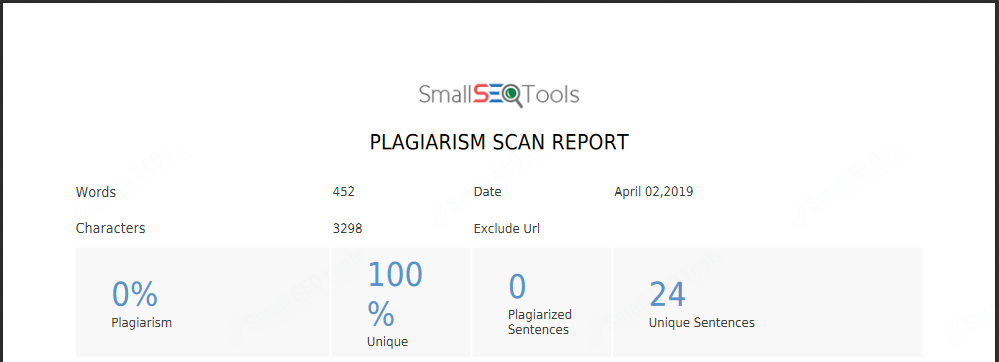
\includegraphics[width=5cm]{figures/5/1174077/teori/plagarismechap5.png}
    \centering
\end{figure}
\end{enumerate}
%%%%%%%%%%%%%%%%%%%%%%%%%%%%%%%%%%%%%%%%%%%%%%%%%%%%%%%%%%%%%%%%%%%%%%%%%%%%%%%%%%%%%%%%%%%%%
\section{Alfadian Owen}
\subsection{Soal 1}
 fungsi device manager di windows dan folder dev di linux.

Device manager digunakan untuk menampilkan seluruh hardware yang bisa di inisialisasi (dikenali) oleh windows.

dev merupakan direktori yang fungsinya untuk menyimpan konfigurasi device atau hardware dari sistem

\subsection{Soal 2}
langkah-langkah instalasi driver dari arduino

\begin{itemize}
	\item Hubungkan port usb Arduino ke port usb pc
	\item Setelah terhubung, di bagian kanan bawah pc anda akan ada notifikasi "installing device driver"
	\item setelah itu akan ada notifikasi gagal menginstall, jangan panik karena memang seperti itu
	\item Buka Device Manager
	\item Di dalam Device Manager cari "unknown device" yang ada di dalam "other device"
	\item Klik kanan lalu update driver software
	\item pilih browse my computer software
	\item cari folder instalan software Arduino yang telah di download
	\item klik next
	\item klik install
	\item selesai
\end{itemize}

\subsection{Soal 3}
cara membaca baudrate dan port

baudrate dan port akan langsung terbaca saat Arduino terpasang ke komputer

\subsection{Soal 4}
sejarah pyserial

Pyserial adalah modul Python API untuk mengakses serial port, Pyserial menyediakan API yang seragam di berbagai sistem operasi termasuk windows,linux,dan BSD

\subsection{Soal 5}
Fungsi yang dipakai dari pyserial

\begin{itemize}
	\item Close()

	untuk menutup port

	\item Write()

	untuk menulis string

	\item Read(byte)

	untuk membaca per byte

	\item Readline()

	untuk membaca sampai line terakhir

	\item Serial()

	untuk membuka port

\end{itemize}
\subsection{Soal 6}
Jelaskan kenapa butuh perulangan dan tidak butuh perulangan dalam membaca serial

Perulangan digunakan untuk membaca data tidak hanya satu kali, dengan adanya perulangan kita dapat membaca data berulang kali. Sehingga data yang dibaca dapat muncul berulang kali.

\subsection{Soal 7}
cara membuat fungsi pyserial

Buat definisi seperti di python dengan menulus “def namafungsi() :”


%%%%%%%%%%%%%%%%%%%%%%%%%%%%%%%%%%%%%%%%%%%%%%%%%%%%%%%%%%%%%%%%%%%%%%%%%%%%%%%%%%%%%%%%%%%%%%%%%%%

\section{Fernando Lorencius S/1174072}
	\subsection{Soal 1} 
		\begin{itemize}
			\item Device Manager : Device Manager menampilkan seluruh hardware yang terinstall dalam komputer atau dikenali oleh Windows.

			\item folder /dev : Dalam sistem operasi Linux, device atau perangkat yang tehubung akan dianggap file.dalam folder /dev terdapat file - file  tersebut berada.
		\end{itemize}

	\subsection{Soal 2}
	Langkah - langkah instalasi driver arduino :
		\begin{enumerate}
			\item sambungkan board Arduino yang dimiliki  ke port USB pada komputer atau laptop, setelah melakukan hal tersebut tunggu hingga Windows mencoba untuk menginstall driver sendiri
			\item setelah melakukan step pertama kita harus memiliki dahulu sofware Arduino, file driver arduino terlebih dahulu dan masukkan ke dalam directory yang terdapat pada komputer diusahakan directory di simpan di file yang mudah di cari
		
			
			\item lalu windows akan memberitahukan notifikasi pop up yang menginformasikan bahwa ingin menginstall dirver, namun nanti biasanya tidak akan menemukan drivernya
			
			\item buka Device Manager ,Klik Start – pilih Control Panel. Di dalam Control Panel, pilih System and Security, lalu pilih System. Selanjutnya pilih Device Manager. 
			\item cari unknown device yang terdapat dalam Device Manager.
			
			\item lakukan klik kanan kepada unknown device tersebut ,setelah itu pilih update driver software
		
			
			\item pilih browse my computer for driver software sesuai dengan directory dalam bagian pertama dalam proses instalisasi
			
			
			\item setelah melakukan proses tersebut, klik install dan tunggu hingga proses selesai
			
			
			\item arduino pun sudah bisa di gunakan dalam komputer / laptop  anda 
			
		\end{enumerate}

	\subsection{Soal 3}
	Untuk mengetahui atau membaca baudrate dan port kita diwajibkan menginstall Arduino IDE, setelah melakukan instalasi atau memiliki Arduino IDE  buka menu serial monitor yang terdapat di dalam tab tools. Dari hasil proses tersebut kita dapat melihat baudrate dan port yang sedang terhubung oleh arduin anda.

	\subsection{Soal 4}
PySerial merupakan paket Python yang memberikan akses atau memberikan memfasilitasi komunikasi serial antara Komputer / laptop dengan perangkat keras eksternal. PySerial menyediakan antarmuka untuk berkomunikasi melalui protokol komunikasi serial. Komunikasi serial merupakan protokol komunikasi komputer tertua. PySerial pertama kali diluncurkan pada tahun 2002 dan makin berkembang dalam setiap versinya hingga tahun 2017 lalu.

	\subsection{Soal 5}
		\begin{itemize}
			\item \begin{verbatim} readline()\end{verbatim} : fungsi serial digunakan untuk menerjemahkan sebuah string dari port serial
			\item \begin{verbatim}Serial(sequence)\end{verbatim} :fungsi serial digunakan untuk membuka port serial.
			\item \begin{verbatim}close()\end{verbatim} : fungsi tersebut digunakan untuk menutup port  dan menghentikan pembacaan program
			\item \begin{verbatim}Write()\end{verbatim} : fungsi write menulis data lewat port serial 
			\item \begin{verbatim}read(size)\end{verbatim}	: fungsi read(size) digunakan membaca seluruh jumlah byte dari port serial.
		\end{itemize}

	\subsection{Soal 6}
	Dalam proses membaca serial di Arduino diperlukan perulangan supaya program dapat membaca data secara berulang kali sehingga data yang muncul banyak.Namun apabila tidak dibutuhkan perulangan maka Arduino akan membaca data cukup sekali saja.

	\subsection{Soal 7}
	Untuk membangun fungsi yang menggunakan pyserial hal yang pertama digunakan kita hanya perlu untuk menginisialisasi pembuatan funsi dengan mengunakan perintah fungsi def namafungsi() : lalu masukan indentasi. atau menggunakan fungsi while loop degan menggunakan  fungsi while true:


%%%%%%%%%%%%%%%%%%%%%%%%%%%%%%%%%%%%%%%%%%%%%%%%%%%%%%%%%%%%%%%%%%%%%%%%%%%%%%%%%%%%%%%%%%%%%%%%%%%

\section{Handi Hermawan}
\subsection{Soal Nomor 1}
Apa itu fungsi device manager di windows dan folder /dev di linux?\\
Jawab :
\begin{itemize}
\item Fungsi Device Manager di Sistem Operasi Windows yaitu
\end{itemize}
Beberapa fungsi kegunaan Device Manager yaitu menunjukkan status suatu hardware, menunjukkan informasi detil suatu hardware, mengelola driver hardware, disable  Enable hardware, meng-identifikasi konflik antar hardware dan Device Manager paling sering digunakan untuk pengelolaan driver suatu hardware. 
\begin{itemize}
\item Fungsi Folder /dev di Sistem Operasi Linux
\end{itemize}
Device manager pada linux berada pada folder /dev yang mempunyai arti device. folder ini berisi konfigurasi device pada sistem.

\subsection{Soal Nomor 2}
Jelaskan langkah-langkah instalasi driver dari arduino!\\
Jawab :
\begin{enumerate}
\item Pertama, Download dan Extract Software Arduino IDE
\item Hubungkan Port USB Arduino UNO ke Port USB PC.
\item Maka PC akan mendeteksi keberadaan perangkat baru.
\item Buka Device Manager dengan mengetik Device Manager di Search Program and Files
\item Setelah Device Manager terbuka, silahkan cari “Unknown Device” yang berada di Other Device.
\item Lalu klik kanan pada Unknown device, pilih Update Driver Software.
\item Pilih Browse my computer for driver software, lalu cari Folder Instalan Software Arduino IDE
\item lalu kilik Next, dan Windowspun akan mencari dan menginstal driver yang berada pada Folder tersebut.
\item Setelah muncul peringatan, klik Install.
\item Selesai, Arduino UNO sudah dikenali oleh PC.
\end{enumerate}

\subsection{Soal Nomor 3}
Jelaskan bagaimana cara membaca baud rate dan port dari komputer yang sudah
terinstall driver! \\
Jawab :\\
Cara membaca baudrate dan port kita hanya perlu menginstall Arduino IDE, setelah itu buka menu serial monitor yang berada di tab tools. Dari sana akan terlihat baudrate dan port yang sedang digunakan oleh arduino.

\subsection{Soal Nomor 4}
Jelaskan sejarah library pyserial!
Jawab : \\
Pyserial akses untuk port serial. Ini menyediakan backends untuk Python berjalan pada Windows, OSX, Linux, BSD (mungkin sistem yang mendukung POSIX) dan IronPython. Modul bernama "serial" secara otomatis memilih backend yang sesuai. PySerial pertama kali diluncurkan pada tahun 2002 yang makin berkembang dalam setiap versinya hingga tahun 2017 lalu.

\subsection{Soal Nomor 5}
Jelaskan fungsi-fungsi apa saja yang dipakai dari library pyserial!\\
Jawab :\\
\begin{itemize}
\item Serial fungsi ini untuk membuka port serial
\item readline berguna untuk membaca sebuah string dari port serial.
\item read(size) berguna untuk membaca jumlah byte dari port serial.
\item close berguna untuk menutup port serial.
\end{itemize}

\subsection{Soal Nomor 6}
Jelaskan kenapa butuh perulangan dan tidak butuh perulangan dalam membaca serial!\\
Jawab :\\
\begin{itemize}
\item Perulangan
\end{itemize}
Dalam perulangan diperlukan untuk untuk mengulangi perintah agar lebih mudah dan tidak terjadi penumpukan kodingan. Perulangan dijalankan jika kondisi benar dan akan berhenti jika kondisi salah.

\begin{itemize}
\item Tidak butuh perulangan
\end{itemize}
Dan apabila perintah dijalankan sekali, kita tidak memerlukan perulangan.

\subsection{Soal Nomor 7}
Jelaskan bagaimana cara membuat fungsi yang menggunakan pyserial!\\
Jawab :\\
Cara membuat fungsi sama seperti pembuatan fungsi seperti biasa namun method dari pyserial dimasukkan kedalam fungsi dan dipanggil fungsi yang kita buat tadi seperti itulah.

\par Scan Plagiarisme
\begin{figure}[ht!]
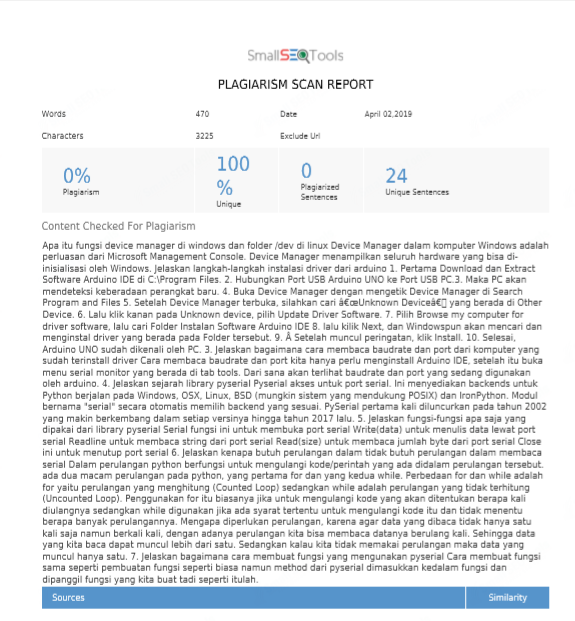
\includegraphics[width=5cm]{figures/5/1174080/Teori/plagiarismteori5.png}
\centering
\caption{plagiarisme}
\end{figure}
%%%%%%%%%%%%%%%%%%%%%%%%%%%%%%%%%%%%%%%%%%%%%%%%%%%%%%%%%%%%%%%%%%%%%%%%%%%%%%%%%%%%%
\section{Muhammad Abdul Gani Wijaya}
{\Large \textbf{Pemahaman Teori}}
\subsection{No. 1}
Device Manager yang ada pada Windows, adalah perluasan dari Microsoft Management Console. Device Manager dapat menampilkan dan mengelola seluruh hardware yang bisa di-inisialisasi (dikenali) oleh Windows. Tampilannya Device Manager telah dikelompokkan sedemikian rupa sehingga akan memudahkan pengelolaan setiap hardware yang ada. Device Manager sangat membantu dalam mengelola (manage) semua hardware yang terpasang dan terdeteksi di dalam Windows. Pada hardware seperti harddisk, kartu VGA, sound, keyboard, perangkat USB dll. akan mudah untuk dikonfigurasi oleh Device Manager ini.
/dev/ : adalah direktori yang berfungsi untuk menyimpan konfigurasi device atau hardware dari system pada linux, seperti harddisk (hda, sda), terminal (tty) etc.

/dev/ : adalah direktori yang berfungsi untuk menyimpan konfigurasi device atau hardware dari system pada linux, seperti harddisk (hda, sda), terminal (tty) etc.

\subsection{No. 2}
Jelaskan langkah-langkah instalasi driver dari arduino!

\hfill \break
Berikut ini adalah langkah-langkah instalasi driver dari Arduino UNO di Windows:

\begin{enumerate}
    \item Pertama double click pada Installer Arduino
    \item Lalu akan muncul License Agreement, klik I Agree
    \begin{figure}[H]
		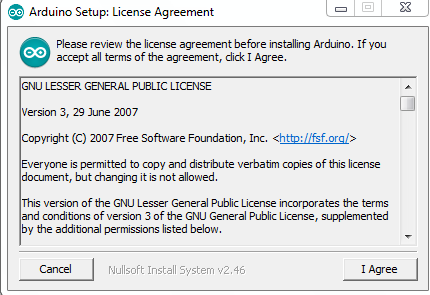
\includegraphics[width=10cm]{figures/5/1174071/Teori/1.png}
		\centering
	\end{figure}
    \item Lalu akan diminta menetukan lokasi instalasi Arduino.
    Anda bisa mengubahnya sesuai keinginan atau membiarkannya tetap default.
    \begin{figure}[H]
		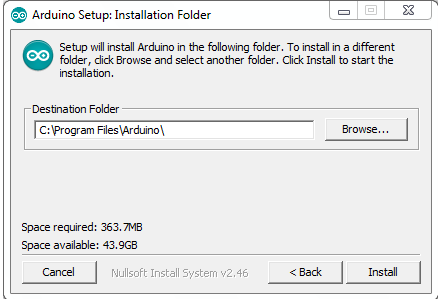
\includegraphics[width=10cm]{figures/5/1174071/Teori/2.png}
		\centering
	\end{figure}
    \item Setelah akan ditampilkan jendela Installation Options. Centang saja semuanya lalu klik next.
    \begin{figure}[H]
		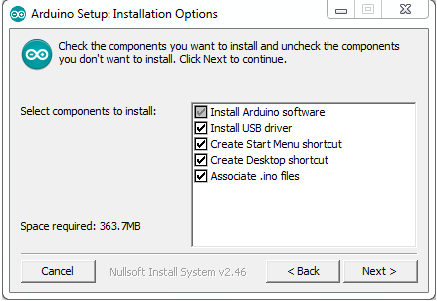
\includegraphics[width=10cm]{figures/5/1174071/Teori/3.png}
		\centering
	\end{figure}
    \item Lalu proses instalasi seperti pada gambar berikut.
    \begin{figure}[H]
		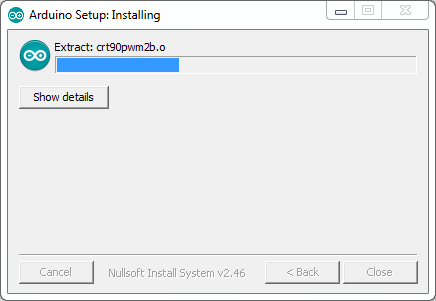
\includegraphics[width=10cm]{figures/5/1174071/Teori/4.png}
		\centering
	\end{figure}
    \item Ditengan installai muncul Security Warning untuk instalasi Arduino USB driver, klik install.
    \begin{figure}[H]
		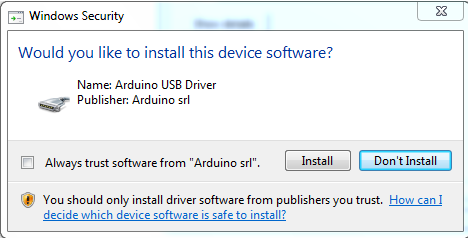
\includegraphics[width=10cm]{figures/5/1174071/Teori/5.png}
		\centering
	\end{figure}
    \item Tunggu sampai installasi complete.
    \begin{figure}[H]
		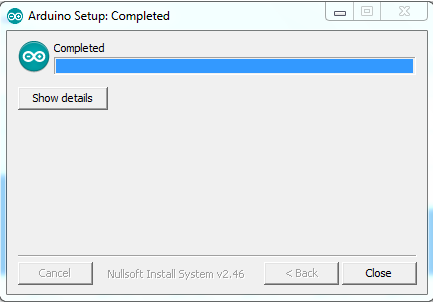
\includegraphics[width=10cm]{figures/5/1174071/Teori/6.png}
		\centering
	\end{figure}
    \item Instalasi Ardunio selesai, dan Arduino Driver siap digunakan.

\end{enumerate}

\subsection{No. 3}
\begin{enumerate}
    \item Pertama buka Device Manager pada laptop
    \item Kemudian klik Ports (COM LPT)
    \item Klik pada Arduino yang terhubung
    \item Klik di tab Port Setting
    \item Di Port Setting ditampilkan Bit Per Second
\end{enumerate}

\subsection{No. 4}
PySerial adalah paket dari Python yang menfasilitasi komunikasi serial antara PC dengan perangkat keras eksternal. PySerial menyediakan antarmuka untuk berkomunikasi melalui protokol komunikasi serial. Komunikasi serial adalah salah satu protokol komunikasi komputer tertua. Protokol komunikasi serial digunakan sebelum adanya USB yang digunakan oleh komputer dan perangkat keras lain seperti mouse, keyboard, dan webcam.

\subsection{Soal No. 5}
\begin{enumerate}
	\item Serial 		: Membuka port serial
	\item Write 		: Menulis data dengan port serial
	\item Readline  	: Membaca port serial
	\item Read	    	: Membaca jumlah byte pada port serial.
	\item Close	    	: Menutup port serial

\end{enumerate}

\subsection{No. 6}
Perulangan diperlukan untuk membaca data berulang terus-menerus untuk menampilkan banyak data. Jika tidak menggunakan perulangan Arduino hanya dapat membaca data satu kali. 

\subsection{No. 7}
Seperti python pada umumnya, fungsi nya dibuat dengan mendeklarasikan def lalu nama fungsinya lalu diikuti dengan isi pada fungsi tersebut.

\subsection{Cek Plagiarisme}
\begin{figure}[H]
		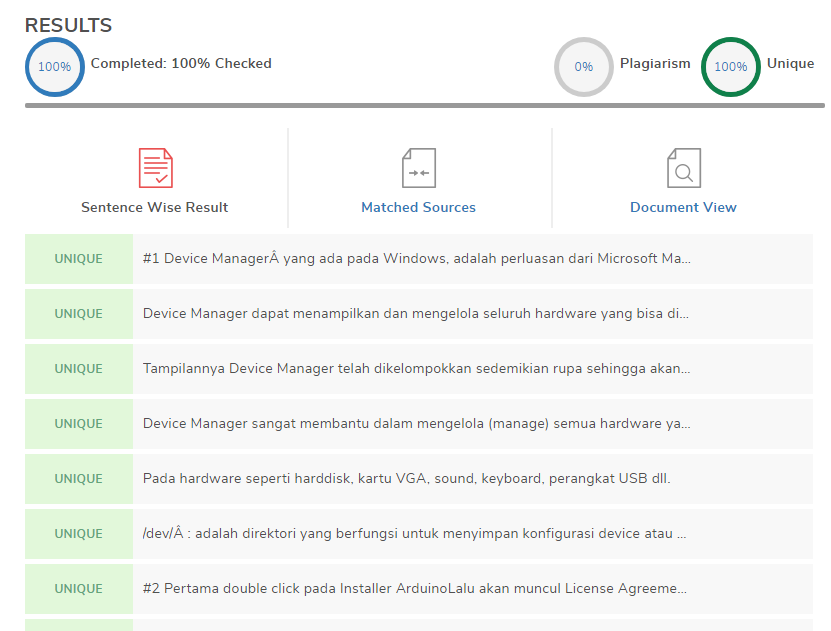
\includegraphics[width=10cm]{figures/5/1174071/Teori/plagiarisme.png}
		\centering
	\end{figure}
%%%%%%%%%%%%%%%%%%%%%%%%%%%%%%%%%%%%%%%%%%%%%%%%%%%%%%%%%%%%%%%%%%%%%%%%%%%%%%%%%%%%%%%%%%